%\RequirePackage{currfile}
\documentclass[12pt]{beamer}
\usepackage[utf8]{inputenc}
\usepackage[spanish]{babel}
\usepackage{standalone}
\usepackage{color}
\usepackage{siunitx}
\usepackage{hyperref}
%\hypersetup{colorlinks,linkcolor=,urlcolor=blue}
%\hypersetup{colorlinks,urlcolor=blue}
\usepackage{xcolor,soul}
\usepackage{etoolbox}
\usepackage{amsmath}
\usepackage{amsthm}
\usepackage{physics}
\usepackage{multicol}
\usepackage{bookmark}
\usepackage{longtable}
\usepackage{listings}
\usepackage{graphicx}
\usepackage{tikz}
\usetikzlibrary{patterns, matrix, backgrounds, decorations,shapes, arrows.meta}
\usepackage[autostyle,spanish=mexican]{csquotes}
\usepackage[os=win]{menukeys}
\usepackage{pifont}
\usepackage{pbox}
\usepackage{caption}
\captionsetup{font=scriptsize,labelfont=scriptsize}
%\usepackage[sfdefault]{roboto}  %% Option 'sfdefault' only if the base font of the document is to be sans serif

%Sección de definición de colores
\definecolor{ao}{rgb}{0.0, 0.5, 0.0}
\definecolor{bisque}{rgb}{1.0, 0.89, 0.77}
\definecolor{amber}{rgb}{1.0, 0.75, 0.0}
\definecolor{armygreen}{rgb}{0.29, 0.33, 0.13}
\definecolor{alizarin}{rgb}{0.82, 0.1, 0.26}
\definecolor{cadetblue}{rgb}{0.37, 0.62, 0.63}
\definecolor{deepblue}{rgb}{0,0,0.5}
\definecolor{brown}{rgb}{0.59, 0.29, 0.0}
\definecolor{OliveGreen}{rgb}{0,0.25,0}


\usefonttheme[onlymath]{serif}
%Sección de definición de nuevos comandos

\newcommand*{\TitleParbox}[1]{\parbox[c]{1.75cm}{\raggedright #1}}%
\newcommand{\python}{\texttt{python}}
\newcommand{\textoazul}[1]{\textcolor{blue}{#1}}
\newcommand{\azulfuerte}[1]{\textcolor{blue}{\textbf{#1}}}
\newcommand{\funcionazul}[1]{\textcolor{blue}{\textbf{\texttt{#1}}}}
\newcommand{\ptilde}[1]{\ensuremath{{#1}^{\prime}}}
\newcommand{\stilde}[1]{\ensuremath{{#1}^{\prime \prime}}}
\newcommand{\ttilde}[1]{\ensuremath{{#1}^{\prime \prime \prime}}}
\newcommand{\ntilde}[2]{\ensuremath{{#1}^{(#2)}}}
\renewcommand{\arraystretch}{1.5}

\newcounter{saveenumi}
\newcommand{\seti}{\setcounter{saveenumi}{\value{enumi}}}
\newcommand{\conti}{\setcounter{enumi}{\value{saveenumi}}}
\renewcommand{\rmdefault}{cmr}% cmr = Computer Modern Roman

\linespread{1.5}

\usefonttheme{professionalfonts}
%\usefonttheme{serif}
\DeclareGraphicsExtensions{.pdf,.png,.jpg}


%Sección para el tema de beamer, con el theme, usercolortheme y sección de footers
\mode<presentation>
{
  \usetheme{Madrid}
  \setbeamertemplate{headline}{}
  %\useoutertheme{infolines}
  \useoutertheme{default}
  \usecolortheme{beaver}
  \setbeamercovered{invisible}
  

  \setbeamertemplate{section in toc}[sections numbered]
  \setbeamertemplate{subsection in toc}[subsections numbered]
  \setbeamertemplate{subsection in toc}{\leavevmode\leftskip=3.2em\rlap{\hskip-2em\inserttocsectionnumber.\inserttocsubsectionnumber}\inserttocsubsection\par}
  \setbeamercolor{section in toc}{fg=blue}
  \setbeamercolor{subsection in toc}{fg=blue}
  \setbeamerfont{subsection in toc}{size=\small}
  \setbeamercolor{frametitle}{fg=blue}

  \setbeamertemplate{navigation symbols}{}
  \setbeamertemplate{caption}[numbered]

  %\beamertemplatenavigationsymbolsempty

  \makeatletter
  \setbeamercolor{section in foot}{bg=green!30!cyan, fg=black!90!orange}
  \setbeamercolor{subsection in foot}{bg=red!30!cyan, fg=red}
  %\setbeamercolor{date in foot}{bg=orange!30!cyan, fg=red}
  \setbeamertemplate{footline}
  {
    \leavevmode%
    \hbox{%
    \begin{beamercolorbox}[wd=.333333\paperwidth,ht=2.25ex,dp=1ex,center]{section in foot}%
      \usebeamerfont{section in foot} \insertsection
    \end{beamercolorbox}}%
    \begin{beamercolorbox}[wd=.333333\paperwidth,ht=2.25ex,dp=1ex,center]{subsection in foot}%
      \usebeamerfont{subsection in foot}  \insertsubsection
    \end{beamercolorbox}%
    \begin{beamercolorbox}[wd=.333333\paperwidth,ht=2.25ex,dp=1ex,right]{date in head/foot}%
      \usebeamerfont{date in head/foot} \insertshortdate{} \hspace*{2em}
      \insertframenumber{} / \inserttotalframenumber \hspace*{2ex} 
    \end{beamercolorbox}}%
    \vskip0pt%

  \makeatother

  \makeatletter
  \patchcmd{\beamer@sectionintoc}
    {\vfill}
    {\vskip\itemsep}
    {}
    {}
  \makeatother
  
}

% Sección para el código

\definecolor{Code}{rgb}{0,0,0}
\definecolor{Keywords}{rgb}{255,0,0}
\definecolor{Strings}{rgb}{255,0,255}
\definecolor{Comments}{rgb}{0,0,255}
\definecolor{Numbers}{rgb}{255,128,0}

\DeclareCaptionFont{white}{\color{white}}
\DeclareCaptionFormat{listing}{\colorbox{gray}{\parbox{0.99\textwidth}{#1#2#3}}}
\captionsetup[lstlisting]{format=listing,labelfont=white,textfont=white}
\renewcommand{\lstlistingname}{Código}

\lstset{
basicstyle=\ttfamily,
columns=fullflexible,
breaklines=true
}

\lstdefinestyle{codigopython}{%
  language=Python,                % choose the language of the code
  %basicstyle=\footnotesize\small,       % the size of the fonts that are used for the code
  numbers=left,                   % where to put the line-numbers
  numberstyle=\scriptsize,      % the size of the fonts that are used for the line-numbers
  stepnumber=1,                   % the step between two line-numbers. If it is 1 each line will be numbered
  numbersep=5pt,                  % how far the line-numbers are from the code
  backgroundcolor=\color{white},  % choose the background color. You must add \usepackage{color}
  showspaces=false,               % show spaces adding particular underscores
  showstringspaces=false,         % underline spaces within strings
  showtabs=false,                 % show tabs within strings adding particular underscores
  frame=single,   		% adds a frame around the code
  tabsize=2,  		% sets default tabsize to 2 spaces
  captionpos=t,   		% sets the caption-position to bottom
  breaklines=true,    	% sets automatic line breaking
  breakatwhitespace=false,    % sets if automatic breaks should only happen at whitespace
  escapeinside={\#},  % if you want to add a comment within your code
  stringstyle =\color{OliveGreen},
  texcl = true,
  %otherkeywords={{as}},             % Add keywords here
  keywordstyle = \color{blue},
  commentstyle = \color{black},
  identifierstyle = \color{black},
  % literate=%
  %         {á}{{\'a}}1
  %         {é}{{\'e}}1
  %         {í}{{\'i}}1
  %         {ó}{{\'o}}1
  %         {ú}{{\'u}}1
  %
  %keywordstyle=\ttb\color{deepblue}
  %fancyvrb = true,
literate={0}{{\textcolor{red}{0}}}{1}%
            {1}{{\textcolor{red}{1}}}{1}%
            {2}{{\textcolor{red}{2}}}{1}%
            {3}{{\textcolor{red}{3}}}{1}%
            {4}{{\textcolor{red}{4}}}{1}%
            {5}{{\textcolor{red}{5}}}{1}%
            {6}{{\textcolor{red}{6}}}{1}%
            {7}{{\textcolor{red}{7}}}{1}%
            {8}{{\textcolor{red}{8}}}{1}%
            {9}{{\textcolor{red}{9}}}{1}%
            {.0}{{\textcolor{red}{.0}}}{2}% Following is to ensure that only periods
            {.1}{{\textcolor{red}{.1}}}{2}% followed by a digit are changed.
            {.2}{{\textcolor{red}{.2}}}{2}%
            {.3}{{\textcolor{red}{.3}}}{2}%
            {.4}{{\textcolor{red}{.4}}}{2}%
            {.5}{{\textcolor{red}{.5}}}{2}%
            {.6}{{\textcolor{red}{.6}}}{2}%
            {.7}{{\textcolor{red}{.7}}}{2}%
            {.8}{{\textcolor{red}{.8}}}{2}%
            {.9}{{\textcolor{red}{.9}}}{2}%
            {\ }{{ }}{1}% handle the space
        ,%
        %mathescape=true
        %escapeinside={*@}
        escapeinside={A_}{_B}
}

%\RequirePackage[l2tabu, orthodox]{nag}
\RequirePackage{currfile}
\documentclass[12pt]{beamer}
\graphicspath{{Imagenes/}{../Imagenes/}}
\usepackage[utf8]{inputenc}
\usepackage[spanish]{babel}
\usepackage{standalone}
\usepackage{color}
\usepackage[binary-units=true]{siunitx}
\usepackage{hyperref}
\hypersetup{
  colorlinks=true,
  linkcolor=blue,          % color of internal links (change box color with linkbordercolor)
  citecolor=green,        % color of links to bibliography
  filecolor=magenta,      % color of file links
  urlcolor=cyan,           % color of external links
  linkbordercolor={0 0 1}
}
\usepackage{xcolor, soul}
\usepackage{etoolbox}
\usepackage{amsmath}
\usepackage{amsthm}
\usepackage{physics}
\usepackage{multicol}
\usepackage{graphicx}
\usepackage{bookmark}
\usepackage{longtable}
\usepackage{graphicx}
\usepackage{tikz}
\usepackage[siunitx, RPvoltages]{circuitikz}
\usetikzlibrary{mindmap}
\usetikzlibrary{arrows, patterns, shapes, decorations.markings, decorations.pathmorphing}
\usetikzlibrary{matrix,positioning}
\tikzstyle{every picture}+=[remember picture,baseline]
\usepackage[autostyle,spanish=mexican]{csquotes}
\usepackage{pifont}
\usepackage[font=footnotesize,textfont=it]{caption}
\usepackage{tabulary}
\usepackage{booktabs}
\usepackage[outdir=./]{epstopdf}
%\usepackage{epstopdf}
\usepackage{media9}
\usepackage{multimedia}
\usepackage{bigints}
%\usepackage{enumitem}
\usepackage[os=win]{menukeys}
\usepackage{pifont}
\usepackage{pbox}
\usepackage{alltt}
\usepackage{verbatim}
\usepackage{colortbl}
\usepackage{tcolorbox}
\usepackage{fancyvrb}
\usepackage[sfdefault]{roboto}  %% Option 'sfdefault' only if the base font of the document is to be sans serif
%\usepackage[T1]{fontenc}
\setcounter{secnumdepth}{3}
\setcounter{tocdepth}{3}
\DeclareGraphicsExtensions{.pdf,.png,.jpg}
\renewcommand {\arraystretch}{1.5}
\definecolor{ao}{rgb}{0.0, 0.5, 0.0}
\definecolor{aquamarine}{rgb}{0.5, 1.0, 0.83}
\definecolor{kellygreen}{rgb}{0.3, 0.73, 0.09}
\definecolor{bisque}{rgb}{1.0, 0.89, 0.77}
\definecolor{amber}{rgb}{1.0, 0.75, 0.0}
\definecolor{armygreen}{rgb}{0.29, 0.33, 0.13}
\definecolor{alizarin}{rgb}{0.82, 0.1, 0.26}
\definecolor{cadetblue}{rgb}{0.37, 0.62, 0.63}
\newcommand*{\TitleParbox}[1]{\parbox[c]{6cm}{\raggedright #1}}%
\newcommand{\python}{\texttt{python}}
\newcommand{\textoazul}[1]{\textcolor{blue}{#1}}
\newcommand{\azulfuerte}[1]{\textcolor{blue}{\textbf{#1}}}
\newcommand{\funcionazul}[1]{\textcolor{blue}{\textbf{\texttt{#1}}}}
%\normalfont
\usepackage{ccfonts}% http://ctan.org/pkg/{ccfonts}
\usepackage[T1]{fontenc}% http://ctan.or/pkg/fontenc
\renewcommand{\rmdefault}{cmr}% cmr = Computer Modern Roman
\usefonttheme[onlymath]{serif}
\linespread{1.3}
\newcounter{saveenumi}
\newcommand{\seti}{\setcounter{saveenumi}{\value{enumi}}}
\newcommand{\conti}{\setcounter{enumi}{\value{saveenumi}}}
\newcommand{\tikzmark}[1]{\tikz[remember picture] \node[coordinate] (#1) {#1};}

\usepackage{scalerel}[2016-12-29]
\def\stretchint#1{\vcenter{\hbox{\stretchto[440]{\displaystyle\int}{#1}}}}
\def\scaleint#1{\vcenter{\hbox{\scaleto[3ex]{\displaystyle\int}{#1}}}}
\def\bs{\mkern-12mu}

\newtheorem{teo}{}[section]
\usepackage{blkarray}

%reduce el tamaño de letra de la etiqueta equations
\makeatletter
\def\maketag@@@#1{\hbox{\m@th\normalfont\small#1}}
\makeatother

%se usa para la x en itemize
\newcommand{\xmark}{\text{\ding{55}}}

%\AtBeginDocument{\setlength{\tymin}{1em}}


\definecolor{myblue}{rgb}{.8, .8, 1}

\usepackage{empheq}

\newlength\mytemplen
\newsavebox\mytempbox

\makeatletter
\newcommand\mybluebox{%
    \@ifnextchar[%]
       {\@mybluebox}%
       {\@mybluebox[0pt]}}

\def\@mybluebox[#1]{%
    \@ifnextchar[%]
       {\@@mybluebox[#1]}%
       {\@@mybluebox[#1][0pt]}}

\def\@@mybluebox[#1][#2]#3{
    \sbox\mytempbox{#3}%
    \mytemplen\ht\mytempbox
    \advance\mytemplen #1\relax
    \ht\mytempbox\mytemplen
    \mytemplen\dp\mytempbox
    \advance\mytemplen #2\relax
    \dp\mytempbox\mytemplen
    \colorbox{myblue}{\hspace{1em}\usebox{\mytempbox}\hspace{1em}}}

\makeatother



%Se usa la plantilla Madrid modificada con beaver
\mode<presentation>
{
  \usetheme{Madrid}
  \setbeamertemplate{headline}{}
  %\useoutertheme{infolines}
  \usecolortheme{beaver}
  \setbeamercovered{invisible}
  

\setbeamertemplate{section in toc}[sections numbered]
\setbeamertemplate{subsection in toc}[subsections numbered]
\setbeamertemplate{subsection in toc}{\leavevmode\leftskip=3.2em\rlap{\hskip-2em\inserttocsectionnumber.\inserttocsubsectionnumber}\inserttocsubsection\par}
\setbeamercolor{section in toc}{fg=blue}
\setbeamercolor{subsection in toc}{fg=blue}
\setbeamerfont{subsection in toc}{size=\small}

\setbeamertemplate{navigation symbols}{}
\setbeamertemplate{caption}[numbered]

}

\usepackage{courier}
\usepackage{listingsutf8}
\usepackage{listings}
\usepackage{xcolor}
\usepackage{textcomp}
\usepackage{color}
\definecolor{deepblue}{rgb}{0,0,0.5}
\definecolor{brown}{rgb}{0.59, 0.29, 0.0}
\definecolor{OliveGreen}{rgb}{0,0.25,0}
% \usepackage{minted}

\DeclareCaptionFont{white}{\color{white}}
\DeclareCaptionFormat{listing}{\colorbox{gray}{\parbox{0.98\textwidth}{#1#2#3}}}
\captionsetup[lstlisting]{format=listing,labelfont=white,textfont=white}
\renewcommand{\lstlistingname}{Código}


\definecolor{Code}{rgb}{0,0,0}
\definecolor{Keywords}{rgb}{255,0,0}
\definecolor{Strings}{rgb}{255,0,255}
\definecolor{Comments}{rgb}{0,0,255}
\definecolor{Numbers}{rgb}{255,128,0}

\makeatletter

\newif\iffirstchar\firstchartrue
\newif\ifstartedbyadigit
\newif\ifprecededbyequalsign

\newcommand\processletter
{%
  \ifnum\lst@mode=\lst@Pmode%
    \iffirstchar%
        \global\startedbyadigitfalse%
      \fi
      \global\firstcharfalse%
    \fi
}

\newcommand\processdigit
{%
  \ifnum\lst@mode=\lst@Pmode%
      \iffirstchar%
        \global\startedbyadigittrue%
      \fi
      \global\firstcharfalse%
  \fi
}

\lst@AddToHook{OutputOther}%
{%
  \lst@IfLastOtherOneOf{=}
    {\global\precededbyequalsigntrue}
    {}%
}

\lst@AddToHook{Output}%
{%
  \ifprecededbyequalsign%
      \ifstartedbyadigit%
        \def\lst@thestyle{\color{orange}}%
      \fi
    \fi
  \global\firstchartrue%
  \global\startedbyadigitfalse%
  \global\precededbyequalsignfalse%
}

\lstset{ 
language=Python,                % choose the language of the code
basicstyle=\footnotesize\ttfamily,       % the size of the fonts that are used for the code
numbers=left,                   % where to put the line-numbers
numberstyle=\scriptsize,      % the size of the fonts that are used for the line-numbers
stepnumber=1,                   % the step between two line-numbers. If it is 1 each line will be numbered
numbersep=5pt,                  % how far the line-numbers are from the code
backgroundcolor=\color{white},  % choose the background color. You must add \usepackage{color}
showspaces=false,               % show spaces adding particular underscores
showstringspaces=false,         % underline spaces within strings
showtabs=false,                 % show tabs within strings adding particular underscores
frame=single,   		% adds a frame around the code
tabsize=2,  		% sets default tabsize to 2 spaces
captionpos=t,   		% sets the caption-position to bottom
breaklines=true,    	% sets automatic line breaking
breakatwhitespace=false,    % sets if automatic breaks should only happen at whitespace
escapeinside={\#},  % if you want to add a comment within your code
stringstyle =\color{OliveGreen},
%otherkeywords={{as}},             % Add keywords here
keywordstyle = \color{blue},
commentstyle = \color{black},
identifierstyle = \color{black},
literate=%
         {á}{{\'a}}1
         {é}{{\'e}}1
         {í}{{\'i}}1
         {ó}{{\'o}}1
         {ú}{{\'u}}1
%
%keywordstyle=\ttb\color{deepblue}
%fancyvrb = true,
}

\lstdefinestyle{FormattedNumber}{%
    literate={0}{{\textcolor{red}{0}}}{1}%
             {1}{{\textcolor{red}{1}}}{1}%
             {2}{{\textcolor{red}{2}}}{1}%
             {3}{{\textcolor{red}{3}}}{1}%
             {4}{{\textcolor{red}{4}}}{1}%
             {5}{{\textcolor{red}{5}}}{1}%
             {6}{{\textcolor{red}{6}}}{1}%
             {7}{{\textcolor{red}{7}}}{1}%
             {8}{{\textcolor{red}{8}}}{1}%
             {9}{{\textcolor{red}{9}}}{1}%
             {.0}{{\textcolor{red}{.0}}}{2}% Following is to ensure that only periods
             {.1}{{\textcolor{red}{.1}}}{2}% followed by a digit are changed.
             {.2}{{\textcolor{red}{.2}}}{2}%
             {.3}{{\textcolor{red}{.3}}}{2}%
             {.4}{{\textcolor{red}{.4}}}{2}%
             {.5}{{\textcolor{red}{.5}}}{2}%
             {.6}{{\textcolor{red}{.6}}}{2}%
             {.7}{{\textcolor{red}{.7}}}{2}%
             {.8}{{\textcolor{red}{.8}}}{2}%
             {.9}{{\textcolor{red}{.9}}}{2}%
             {\ }{{ }}{1}% handle the space
         ,%
          %mathescape=true
          escapeinside={__}
          }



\makeatletter
\setbeamercolor{section in foot}{bg=green!30!cyan, fg=black!90!orange}
\setbeamercolor{subsection in foot}{bg=red!30!cyan, fg=red}
%\setbeamercolor{date in foot}{bg=orange!30!cyan, fg=red}
\setbeamertemplate{footline}
{
  \leavevmode%
  \hbox{%
  \begin{beamercolorbox}[wd=.333333\paperwidth,ht=2.25ex,dp=1ex,center]{section in foot}%
    \usebeamerfont{section in foot} \insertsection
  \end{beamercolorbox}}%
  \begin{beamercolorbox}[wd=.333333\paperwidth,ht=2.25ex,dp=1ex,center]{subsection in foot}%
    \usebeamerfont{subsection in foot}  \insertsubsection
  \end{beamercolorbox}%
  \begin{beamercolorbox}[wd=.333333\paperwidth,ht=2.25ex,dp=1ex,right]{date in head/foot}%
    \usebeamerfont{date in head/foot} \insertshortdate{} \hspace*{2em}
    \insertframenumber{} / \inserttotalframenumber \hspace*{2ex} 
  \end{beamercolorbox}}%
  \vskip0pt%
\makeatother
\title{Integración numérica}
\subtitle{Tema 2 - Operaciones matemáticas básicas}
\author{M. en C. Gustavo Contreras Mayén}
\date{\today}
\institute{Facultad de Ciencias - UNAM}
\titlegraphic{
\includegraphics[width=1.75cm]{Imagenes/escudo-facultad-ciencias}\hspace*{4.75cm}~%
   
\includegraphics[width=1.75cm]{Imagenes/escudo-unam}
}
\begin{document}
\maketitle
\fontsize{14}{14}\selectfont
\spanishdecimal{.}
\section*{Contenido}
\frame{\tableofcontents[currentsection, hideallsubsections]}
\section{Integración numérica}
\frame{\tableofcontents[currentsection, hideothersubsections]}
\subsection{Problema inicial}
\begin{frame}
\frametitle{Problema inicial}
La integración numérica es ciertamente uno de los conceptos más importantes en el análisis computacional, ya que juega un papel importante en el tratamiento numérico de las ecuaciones diferenciales.
\end{frame}
\begin{frame}
\frametitle{Problema inicial}
Dada una función $f(x)$ que es continua en el intervalo $[a, b]$, uno desea aproximar la integral
\begin{align*}
\int_{a}^{b} f(x) \dd{x}
\end{align*}
\end{frame}
\section{Introducción}
\frame{\tableofcontents[currentsection, hideothersubsections]}
\subsection{Base de la integración numérica}
\begin{frame}
\frametitle{Introducción}
La integración numérica (también conocida como \textcolor{blue}{cuadratura}) es un procedimiento con mayor precisión que la diferenciación numérica.
\end{frame}
\begin{frame}
\frametitle{Introducción}
La cuadratura aproxima la integral definida
\begin{align*}
\int_{a}^{b} f(x) \dd{x}
\end{align*}
mediante la suma
\begin{align*}
I = \sum_{i=0}^{n} A_{i} \, f(x_{i})
\end{align*}
\end{frame}
\begin{frame}
\frametitle{Introducción}
\begin{align*}
I = \sum_{i=0}^{n} A_{i} \, f(x_{i})
\end{align*}
donde las \textit{abscisas nodales} $x_{i}$ y los pesos $A_{i}$ dependen de una regla en particular usada para la cuadratura.
\end{frame}
\begin{frame}
\frametitle{Clasificación de las cuadraturas}
Todas las reglas de cuadratura se dividen en dos grupos:
\setbeamercolor{item projected}{bg=blue!70!black,fg=yellow}
\setbeamertemplate{enumerate items}[circle]
\begin{enumerate}[<+->]
\item Fórmulas de \textcolor{red}{Newton-Cotes}.
\item Fórmulas de \textcolor{blue}{Cuadraturas Gaussianas}.
\end{enumerate}
\end{frame}
\section{Fórmulas de Newton-Cotes}
\frame{\tableofcontents[currentsection, hideothersubsections]}
\subsection{Definición de las fórmulas}
\begin{frame}
\frametitle{Fórmulas de Newton-Cotes}
Estas fórmulas se caracterizan por usar un \textcolor{red}{espaciamiento uniforme y constante en las abscisas}, aquí se consideran los métodos:
\begin{itemize}
\item Del trapecio.
\item La regla de Simpson.
\end{itemize}
\end{frame}
\begin{frame}
\frametitle{Fórmulas de Newton-Cotes}
Son útiles si $f(x)$ se ha evaluado en intervalos iguales; dado que \emph{las fórmulas Newton-Cotes se basan en una interpolación local}, se requiere de una porción del dominio para ajustarla al polinomio.
\end{frame}
\begin{frame}
\frametitle{Fórmulas de Cuadraturas Gaussianas}
En la Cuadratura Gaussiana, las posiciones de las abscisas se eligen para obtener la mejor precisión posible.
\\
\bigskip
Debido a que la Cuadratura Gaussiana requiere menos evaluaciones del integrando para un nivel de precisión dado.
\end{frame}
\begin{frame}
\frametitle{Fórmulas de Cuadraturas Gaussianas}
Esta técnica es más popular en los casos en los que para evaluar $f(x)$, implica un costo computacional más elevado.
\end{frame}
\begin{frame}
\frametitle{Fórmulas de Cuadraturas Gaussianas}
\renewcommand\familydefault{lmr}
Otra ventaja de la Cuadratura Gaussiana es su capacidad para manejar singularidades integrables, lo que permite evaluar expresiones como
\begin{equation*}
\bigints\limits_{0}^{1} \dfrac{g(x)}{\sqrt{1 - x^{2}}} \dd{x}
\end{equation*}
siempre que la $g(x)$ sea una función \emph{bien comportada}.
\end{frame}
\begin{frame}
\frametitle{Fórmulas de Newton-Cotes}
Consideremos la integral definida
\begin{align*}
\int_{a}^{b} f(x) \dd{x}
\end{align*}
Dividimos el intervalo de integración $[a,b]$ en $n$ intervalos de igual longitud $h = (b-a)/n$, y hacemos que las abscisas sean $x_{0}, x_{1}, \ldots, x_{n}$.
\end{frame}
\begin{frame}
\frametitle{Aproximación polinomial de $f(x)$}
	\begin{figure}
		\centering
		\includestandalone{Figuras/integracion_01}
		\caption{Aproximación polinomial para la función.}
	\end{figure}
\end{frame}
\begin{frame}
\frametitle{Aproximación polinomial de $f(x)$}
Ahora aproximamos $f(x)$ con un polinomio de orden $n$ que intersecta todos los nodos.
\\
\bigskip
\pause
La expresión para el polinomio de Lagrange es:
\begin{align*}
P_{n}(x) = \sum_{i=0}^{n} f(x_{i}) \, \mathcal{L}_{i}(x)
\end{align*}
donde $\mathcal{L}_{i}(x)$ son las funciones definidas en el tema de interpolación. 
\end{frame}
\begin{frame}
\frametitle{Aproximación polinomial de $f(x)$}
Por tanto, un aproximación a la integral es
\begin{align*}
I = \int_{a}^{b} P_{n}(x) \dd{x} &= \sum_{i=0}^{n} \left[ f(x_{i}) \, \int_{a}^{b} \, \mathcal{L}_{i}(x) \dd{x} \right] = \\[0.5em]
&= \sum_{i=0}^{n} A_{i} \, f(x_{i})
\end{align*}
donde
\begin{align*}
A_{i} = \int_{a}^{b} \mathcal{L}_{i} \dd{x}, \hspace{1cm} i = 0, 1, \ldots, n
\end{align*}
\end{frame}
\begin{frame}
\frametitle{Fórmulas de Newton-Cotes}
Las ecuaciones
\fontsize{12}{12}\selectfont
\begin{align*}
I = \int_{a}^{b} P_{n}(x) \dd{x} = \sum_{i=0}^{n} \left[ f(x_{i}) \, \int_{a}^{b} \mathcal{L}_{i}(x) \dd{x} \right] = \sum_{i=0}^{n} A_{i} \, f(x_{i})
\end{align*}
\fontsize{14}{14}\selectfont
\pause
se conocen como las \emph{fórmulas de Newton-Cotes}.
\end{frame}
\begin{frame}
\frametitle{Fórmulas de Newton-Cotes}
Dependiendo del valor de $n$ tendremos los siguientes casos:
\setbeamercolor{item projected}{bg=blue!70!black,fg=yellow}
\setbeamertemplate{enumerate items}[circle]
\begin{enumerate}[<+->]
\item $n = 1$, Regla del trapecio.
\item $n = 2$, Regla de Simpson.
\item $n = 3$, Regla de Simpson de $3/8$.
\end{enumerate}
\end{frame}
\begin{frame}
\frametitle{Fórmulas de Newton-Cotes}
La más importante es la regla del trapecio, ya que se puede combinar con la extrapolación de Richardson, en un algoritmo eficiente llamado: \textcolor{blue}{Integración de Romberg}.
\end{frame}
\subsection{Regla del trapecio}
\begin{frame}
\frametitle{Regla del trapecio}
Con $n = 1$ se genera un panel como el que se muestra a continuación:
\begin{figure}
	\centering
	\includestandalone{Figuras/integracion_02}
\end{figure}
\end{frame}
\begin{frame}
\frametitle{Regla del trapecio}
El espacio $E$ representa el error debido a la aproximación, la línea azul es $f(x)$ y la aproximación a la integral es $I$.
\begin{figure}
    \centering
    \includestandalone{Figuras/integracion_02}
\end{figure}
\end{frame}    
\begin{frame}
\frametitle{Regla del trapecio}
De acuerdo a la expresión anterior:
\begin{align*}
I = \sum_{i=0}^{1} A_{i} \, f(x_{i}) = A_{0} \, f(x_{0}) + A_{1} \, f(x_{1})
\end{align*}
donde
\begin{align*}
A_{0} = \int_{a}^{b} \ell_{0} \dd{x}, \hspace{1.5cm} A_{1} = \int_{a}^{b} \ell_{1} \dd{x}
\end{align*}
\end{frame}
\begin{frame}
\frametitle{Regla del trapecio}
Se tiene entonces que 
\begin{align*}
l_{0} = \dfrac{(x-x_{1})}{(x_{0}-x_{1})} = \dfrac{(x-b)}{h}
\end{align*}
por tanto:
\begin{align*}
A_{0} = \dfrac{1}{h} \, \int_{a}^{b} (x - b) \dd{x} = \dfrac{1}{2 \, h} \, (b - a)^{2}= \dfrac{h}{2}
\end{align*}
\end{frame}
\begin{frame}
\frametitle{Regla del trapecio}
Ahora se calcula el valor para
\begin{align*}
l_{1} = \dfrac{(x - x_{0})}{(x_{1} - x_{0})} = \dfrac{(x-a)}{h}
\end{align*}
por lo que tenemos
\begin{align*}
A_{1} = \dfrac{1}{h} \, \int_{a}^{b} (x - a) \dd{x} = \dfrac{1}{2h} \, (b - a)^{2}= \dfrac{h}{2}
\end{align*}
\end{frame}
\begin{frame}
\frametitle{Regla del trapecio}
Sustituyendo entonces obtenemos el valor de la integral de $f(x)$ en $[a, b]$:
\begin{align*}
I = \left[ f(a) + f(b) \right] \, \dfrac{h}{2}
\end{align*}
\end{frame}
\begin{frame}
\frametitle{Regla del trapecio}
\begin{figure}
	\centering
	\includestandalone{Figuras/integracion_02}
\end{figure}
Que resulta ser la regla del trapecio, y representa el área del trapecio que se muestra en la figura.
\end{frame}
\subsection{Error en la regla del trapecio}
\begin{frame}
\frametitle{Error en la regla del trapecio}
El error debido a la aproximación viene dado por
\begin{align*}
E = \int_{a}^{b} f(x) \dd{x} - I
\end{align*}
que es diferencia entre el área debajo de la curva de $f(x)$ y el valor de la integral obtenida. 
\end{frame}
\begin{frame}
\frametitle{Error en la regla del trapecio}
Integrando el error de interpolación:
\begin{align*}
E &= \dfrac{1}{2!} \: \int_{a}^{b} (x - x_{0})(x - x_{1}) \: f^{\prime \prime}(\xi) \: \dd{x}  \\
&= \dfrac{1}{2} \: f^{\prime \prime}(\xi) \: \int_{a}^{b} (x - a)(x - b) \: \dd{x} = \\
&= -\dfrac{1}{12}(b - a)^{3} f^{\prime \prime} (\xi) \\
&= -\dfrac{h^{3}}{12} \: f^{\prime \prime}(\xi)
\end{align*}
\end{frame}
\begin{frame}
\frametitle{Error en la regla del trapecio}
Vemos que el error es proporcional a $h^{3}$ y a la segunda derivada de $f(x)$, por lo que ya podremos estimar numéricamente el valor del error, recordemos que $\xi$ no es un valor que conozcamos de manera explícita pero buscaremos minimizarlo y así obtener un valor de error ponderado.
\end{frame}
\subsection{Regla extendida del trapecio}
\begin{frame}
\frametitle{Regla extendida del trapecio}
En la práctica la regla del trapecio se usa con una sola división en el dominio.
\end{frame}
\begin{frame}
\frametitle{Regla extendida del trapecio}
La siguiente figura muestra el dominio $[a,b]$ dividido en $n$ bloques, cada uno de longitud $h$.
\begin{figure}
	\centering
	\includestandalone[scale=1.2]{Figuras/integracion_03}
\end{figure}
\end{frame}
\begin{frame}
\frametitle{Regla extendida del trapecio}
La función $f(x)$ se integrará con una aproximación lineal en cada panel. 
\\
\bigskip
\pause
De la regla del trapecio, sabemos que para el i-ésimo panel:
\begin{align*}
I_{i} = [ f(x_{i}) + f(x_{i+1}) ] \, \dfrac{h}{2}
\end{align*}
\end{frame}
\begin{frame}
\frametitle{Regla extendida del trapecio}
El área total queda representada por la integral:
\begin{align*}
I \simeq \sum_{i=0}^{n-1} [f(x_{0}) &+ 2 \, f(x_{1}) + 2 \, f(x_{2}) + \ldots + \\ 
&+ 2 \, f(x_{n-1}) + f(x_{n})] \dfrac{h}{2}
\end{align*}
que es la regla del extendida del trapecio.
\end{frame}
\begin{frame}
\frametitle{Error en la regla extendida}
El error de truncamiento para el área de un panel es:
\begin{align*}
E_{i} = - \dfrac{h^{3}}{12} f^{\prime \prime} (\xi_{i})
\end{align*}
donde $\xi_{i}$ se encuentra en $(x_{i}, x_{i+1})$.
\end{frame}
\begin{frame}
\frametitle{Error en la regla extendida}
Por lo que el error de truncamiento es
\begin{align*}
E = \sum_{i=0}^{n-1} E_{i} = - \dfrac{h^{3}}{12} \, \sum_{i=0}^{n-1} f^{\prime \prime} (\xi_{i})
\end{align*}
\pause
Pero
\begin{align*}
\sum_{i=0}^{n-1} f^{\prime \prime} (\xi_{i}) = n \, \overline{f}^{\prime \prime}
\end{align*}
donde $\overline{f}^{\prime \prime}$ es la media aritmética de la segunda derivada.
\end{frame}
\begin{frame}
\frametitle{Error en la regla extendida}
Si $f^{\prime \prime} (x)$ es continua, debe de haber un punto $\xi$ en $(a, b)$ en el que ${f}^{\prime \prime}(\xi) = \overline{f}^{\prime \prime}$.
\\
\bigskip
\pause
Lo que nos permite escribir
\begin{align*}
\sum_{i=0}^{n-1} f^{\prime \prime} (\xi_{i}) = n \, f^{\prime \prime} (\xi) = \dfrac{b-a}{h} \, f^{\prime \prime} (\xi)
\end{align*}
\end{frame}
\begin{frame}
\frametitle{Error en la regla extendida}
Entonces el error $E$ se convierte en
\begin{align*}
E = - \dfrac{(b -a) \, h^{2}}{12} \, f^{\prime \prime} (\xi)
\end{align*}
\pause
Pero sería incorrecto concluir que el valor de $E$ es de la forma $E = c \, h^{2}$ donde $c$ es una constante, ya que $f^{\prime \prime} (\xi)$ no es del todo independiente de $h$.
\end{frame}
\begin{frame}
\frametitle{Error en la regla extendida}
Con un análisis más profundo del error, nos dice que si $f(x)$ y sus derivadas son finitas en el intervalo $(a, b)$, entonces
\begin{align*}
E = c_{1} \, h^{2} + c_{2} \, h^{4} + c_{3} \, h^{6} + \ldots 
\end{align*}
\end{frame}
% \subsection{Regla recursiva del trapecio}
% \begin{frame}
% \frametitle{Regla recursiva del trapecio}
% Sea $I_{k}$ la integral evaluada con la regla compuesta del trapecio, usando $2^{k-1}$ bloques. Con la notación $H=b-a$,de la regla compuesta del trapecio, para $k=1,2,3$
% \[
% 	\begin{split}
% 		k = 1 \text{ (1 bloque) }: \\
% 		I_{1} = [f(a) + f(b)] \frac{H}{2}
% 	\end{split}
% \]
% \end{frame}
% \begin{frame}
% \frametitle{Regla recursiva del trapecio}
% \[
% 	\begin{split}
% 		k = 2 \text{ (2 bloques) }: \\
% 		I_{2} =& \left[ f(a) + 2 \: f\left(a+\frac{H}{2} \right) + f(b) \right] \frac{H}{4} \\
% 		=& \frac{1}{2} \: I_{1} + f \left( a + \frac{H}{2} \right) \: \frac{H}{2}
% 	\end{split}
% \]
% \end{frame}
% \begin{frame}
% \frametitle{Regla recursiva del trapecio}
% \[
% 	\begin{split}
% 		k = &3 \text{ (4 bloques) }: \\
% 		I_{3} =& \left[ f(a) + 2 \: f \left(a + \frac{H}{4} \right) + 2 \: f \left( a + \frac{H}{2} \right) + \right.\\
% 		 +& \left. 2 \: f \left( a + \frac{3 \: H}{4} \right) + f(b) \right] \frac{H}{8} \\
% 		=& \frac{1}{2} \: I_{2} \left[f\left(a+\frac{H}{4} \right) + f\left(a+\frac{3 \: H}{4}\right) \right] \: \frac{H}{4}
% 	\end{split}
% \]
% \end{frame}
% \begin{frame}
% \frametitle{Regla recursiva del trapecio}
% Para un $k > 1$ arbitrario, tenemos
% \[ I_{k} = \dfrac{1}{2} \: I_{k - 1} + \dfrac{H}{2^{k - 1}} \sum_{i = 1}^{2^{k - 2}} \: f \left[ a + \dfrac{(2 \: i - 1)H}{2^{k - 1}} \right], \hspace{0.6cm} k=2,3,\ldots\]
% Otra forma de la misma ecuación es:
% \[ I(h) = \dfrac{1}{2} \: I(2 \: h) + h \sum f(x_{\text{nuevo}}) \]
% \end{frame}
\begin{frame}
\frametitle{Ejercicio}
El cuerpo de revolución que se muestra en la siguiente figura, se obtiene al girar la curva dada por
\begin{align*}
y = 1 + \left( \dfrac{x}{2} \right)^{2}, \hspace{0.5cm} 0 \leq x \leq 2
\end{align*}
en torno al eje $x$.
\end{frame}
\begin{frame}
\frametitle{Figura para el ejercicio}
\begin{figure}
	\centering
	\includestandalone{Figuras/integracion_04}
\end{figure}
\end{frame}
\begin{frame}
\frametitle{Ejercicio}
Calcula el volumen del sólido, usando la regla extendida del trapecio con $N = 2, 4, 8, 16, 32, 64, 128$.
\\
\bigskip
El valor exacto del volumen es es $I = 11.7286$. Evalúa el error que se obtiene para cada $N$.
\end{frame}
\begin{frame}
\frametitle{Resolviendo el problema}
Hay que definir inicialmente la función que queremos integrar, por tanto
\begin{align*}
I = \int_{a}^{b} f(x) \dd{x}
\end{align*}
donde
\begin{align*}
f(x) = \pi \, \left( 1 + \left( \dfrac{x}{2} \right)^{2} \right)^{2}
\end{align*}
\end{frame}
\begin{frame}
\frametitle{Código para la regla extedida}
El siguiente código implementa la regla extendida del trapecio, en donde se requieren los siguientes argumentos:
\setbeamercolor{item projected}{bg=blue!70!black,fg=yellow}
\setbeamertemplate{enumerate items}[circle]
\begin{enumerate}[<+->]
\item La función $f(x)$ que se desea integrar.
\item El intervalo de integración $[a, b]$
\item El número de paneles $n$ en la regla extendida del trapecio.
\end{enumerate}
\end{frame}
\begin{frame}[allowframebreaks, fragile]
\begin{lstlisting}[caption=Código para la función trapecios, style=FormattedNumber, basicstyle=\linespread{1.1}\ttfamily=\small, columns=fullflexible]
def trapecios(f, a, b, n):
   h = (b - a)/float(n)
   x = a
   suma = 0
   
   for i in range(1, n):
      x = x + h
      suma = suma + funcion(x)
   
   return (h/2.) * (funcion(a) + funcion(b) + 2 * suma)

def funcion(x):
   return pi * (1 + (x/2)**2)**2
\end{lstlisting}
\end{frame}
\begin{frame}
\frametitle{Valores de $N$}
Como el enunciado pide que se modifique el valor de $n$, podemos entonces usar una operación básica para que se realice la integración mediante un ciclo \funcionazul{for}.
\\
\bigskip
Damos por hecho de que ya cuentan con una función que evalúe el error relativo, llamada \funcionazul{error\_relativo}.
\end{frame}
\begin{frame}[fragile]
\frametitle{Ejercicio completo}
\begin{lstlisting}[caption=Completamos el código y evaluamos el error, style=FormattedNumber, basicstyle=\linespread{1.1}\ttfamily=\small, columns=fullflexible]
print("i \t Integral \t Error")
print("--"*20)
for i in range(1, 8):
    n = 2**i
    integral = trapecios(funcion(i), 0, 2, n)
    print ('{0:3d} \t {1:2.9f} \t  {3:1.8e}'.format(n, integral, \
                    (error_relativo(integral))))
\end{lstlisting}
\end{frame}
\begin{frame}
\frametitle{Observación}
Nótese que la manera en que incrementamos el valor de $n$, es más dinámica: si aumentamos el número de elementos, tendríamos que ajustar \enquote{a mano} el contenido de una lista.
\\
\bigskip
Hacerlo con un incremento en la potencia, nos permite entonces, manejar cualquier cambio en el número de elementos sin problema ni ajustes manuales.
\end{frame}
\begin{frame}
\frametitle{Tabla de resultado}
\fontsize{12}{12}\selectfont
\begin{center}
\begin{tabular}{r | l | l} 
$i$ & Integral & Error \\ \hline
$2$ & $12.762720155$ & $8.81708094e-00$ \\ \hline
$4$ & $11.989593838$ & $2.22527700e-00$ \\ \hline
$8$ & $11.794011288$ & $5.57707550e-01$ \\ \hline
$16$ & $11.744971839$ & $1.39589033e-01$ \\ \hline
$32$ & $11.732702989$ & $3.49827695e-02$ \\ \hline
$64$ & $11.729635215$ & $8.82641387e-03$ \\ \hline
$128$ & $11.728868236$ & $2.28702562e-03$
\end{tabular}
\end{center}
\end{frame}
\section{Librería Scipy}
\frame{\tableofcontents[currentsection, hideothersubsections]}
\subsection{¿Qué es scipy?}
\begin{frame}
\frametitle{Librería Scipy}
\funcionazul{SciPy} (Scientific Python) es una librería matemática con funciones que extienden la librería \funcionazul{numpy} para \python.
\\
\bigskip
Se le proporciona al usuario un poder significativo mediante el uso de comandos de alto nivel y clases, para la manipulación y visualización de datos.
\end{frame}
% \subsection{Organización de Scipy}
% \begin{frame}
% \frametitle{Organización de Scipy}
% La librería \funcionazul{SciPy} está organizada en sub-paquetes que cubren diferentes áreas de computación científica. Estos se resumen en la siguiente tabla:
% \fontsize{12}{12}\selectfont
% \begin{tabular}{l | l}
% 	Subpaquete	&	Descripción \\ \hline
% 	cluster		&	Algortimos para clusters \\ \hline
% 	constants	&	Constantes físicas y matemáticas \\ \hline
% 	fftpack 	&	Rutinas para la Transformada Rápida de Fourier \\ \hline
% 	integrate	&	Integración y EDO \\ \hline
% 	interpolate	&	Interpolación y uso de splines \\ \hline
% 	io			&	Rutinas de entrada y salida
% \end{tabular}
% \end{frame}
% \begin{frame}
% \fontsize{12}{12}\selectfont
% \begin{tabular}{l | l}
% 	Subpaquete	&	Descripción \\ \hline
% 	linalg		&	Algebra lineal \\ \hline
% 	ndimage		&	Procesamiento N-dimensional de imagenes \\ \hline
% 	odr			&	Regresión de distancias ortogonales \\ \hline
% 	optimize	&	Optimizació y rutinas para encontrar raíces \\ \hline
% 	signal		&	Procesamiento de señales \\ \hline
% 	sparse		&	Matrices sparse y rutinas asociadas \\ \hline
% 	spatial		&	Estructura de datos espaciales \\ \hline
% 	special		&	Funciones especiales \\ \hline
% 	stats		&	Distribuciones estadísticas \\ \hline
% 	weave		&	Integración con C/C++
% \end{tabular}
% \end{frame}
% \subsection{\texttt{scipy.integrate}}
% \begin{frame}
% \frametitle{Integración (\texttt{scipy.integrate})}
% El subpaquete \funcionazul{scipy.integrate} proporciona varias técnicas de integración.
% \fontsize{12}{12}\selectfont
% 	\begin{tabular}{l | p{8cm}}
% 	quad 		& Integración en general. \\ \hline
% 	dblquad 	& Integración doble en general. \\ \hline
% 	tplquad 	& Integración triple en general. \\ \hline
% 	fixed-quad 	& Integración de f(x) usando cuadraturas gaussianas de orden n. \\ \hline
% 	quadrature 	& Integra con tolerancia dada usando cuadratura gaussiana. \\ \hline
% 	romberg 	& Integra una función mediante la integración de Romberg.
% \end{tabular}
% \end{frame}
% \begin{frame}[fragile]
% \frametitle{Usando \funcionazul{integrate.quad}}
% Para comparar el resultado que nos devuelve la función \funcionazul{arg}{scipy.integrate.quad}, veamos cómo implementar la solución del problema del sólido de revolución.
% \end{frame}
% \begin{frame}[fragile]
% \frametitle{Usando \funcionazul{integrate.quad}}
% \begin{lstlisting}[caption=Integración con scipy, style=FormattedNumber, basicstyle=\linespread{1.1}\ttfamily=\small, columns=fullflexible]
% from numpy import pi
% from scipy.integrate import quad

% def f(x):
%     return pi*(1 + (x/2)**2)**2
   
% print(quad(f, 0, 2))
% \end{lstlisting}
% \pause
% El resultado que nos devuelve es: $(11.728612573401893, 1.302137572589889e-13)$.
% \end{frame}
% \begin{frame}[fragile]
% \frametitle{Usando \funcionazul{integrate.quad}}
% El valor posterior al resultado de la integral es el error asociado al algoritmo que usa \funcionazul{integrate.quad}, para que no lo reporte en el resultado, basta con indicar que queremos sólo el primer elemento de la lista:
% \\
% \bigskip
% \verb|print(quad(f, 0, 2)[0])|
% \end{frame}
\section{Reglas de Simpson}
\frame{\tableofcontents[currentsection, hideothersubsections]}
\subsection{Regla de \texorpdfstring{$1/3$}{1/3} de Simpson}
\begin{frame}
\frametitle{Regla de $1/3$ de Simpson}
La regla de $1/3$ de Simpson se obtiene de las fórmulas de Newton-Cotes con $n = 2$.
\\
\bigskip
Mediante una interpolación con una parábola a través de tres nodos, como se muestra en la siguiente figura:
\end{frame}
\begin{frame}
\frametitle{Regla de $1/3$ de Simpson}
\begin{figure}
	\centering
	\includestandalone[scale=0.9]{Figuras/integracion_05}
\end{figure}
El área debajo de la curva representa una aproximación a la integral
\begin{align*}
\int_{a}^{b} f(x) \dd{x}
\end{align*}
\end{frame}
\begin{frame}
\frametitle{Regla de $1/3$ de Simpson}
Es decir
\begin{align*}
\int_{a}^{b} f(x) \dd{x} = I = \left[ f(a) + 4 \: f \left( \dfrac{a + b}{2} \right) + f(b) \right] \: \dfrac{h}{3}
\end{align*}
\end{frame}
\subsection{Regla compuesta de \texorpdfstring{$1/3$}{1/3} de Simpson}
\begin{frame}
\frametitle{Regla compuesta de $1/3$ de Simpson}
Para obtener la regla compuesta de $1/3$ de Simpson, se divide el intervalo de integración $[a, b]$ en $n$ bloques ($n$ par) de ancho $h = (b - a)/n$
\end{frame}
\begin{frame}
\frametitle{Regla compuesta de $1/3$ de Simpson}
\begin{figure}
	\centering
	\includestandalone[scale=1.2]{Figuras/integracion_06}
\end{figure}
\end{frame}
\begin{frame}
\frametitle{Regla compuesta de $1/3$ de Simpson}
Aplicando la fórmula anterior a dos bloques adyacentes, tenemos que:
\begin{align*}
\int_{x_{i}}^{x_{i + 2}} \: f(x) \: \dd{x} \simeq \bigg[ f(x_{i}) + 4 \: f(x_{i + 1}) + f(x_{i + 2}) \bigg] \: \dfrac{h}{3}
\end{align*}
\end{frame}
\begin{frame}
\frametitle{Regla compuesta de $1/3$ de Simpson}
Sustituyendo la ecuación en todo el intervalo
\begin{align*}
\int_{a}^{b} \: f(x) \: \dd{x} &= \int_{x_{0}}^{x_{m}} \: f(x) \: \dd{x} = \\
&= \sum_{i = 0, 2,\ldots}^{n} \left[ \int_{x_{i}}^{x_{i + 2}} \: f(x) \: \dd{x} \right]
\end{align*}
\end{frame}
\begin{frame}
\frametitle{Regla compuesta de $1/3$ de Simpson}
Por lo que la aproximación a la integral resulta ser:
\begin{align*}
\int_{a}^{b} f(x) \dd{x} &\simeq I = \bigg[ f(x_{0}) + 4 \: f(x_{1}) + 2 \: f(x_{2}) + \ldots  \\
& \ldots + 2 \: f(x_{n-2}) + 4 \: f(x_{n - 1}) + f(x_{n}) \bigg] \: \dfrac{h}{3}
\end{align*}
\pause
y es quizás el método más conocido de integración numérica. 
\end{frame}
\begin{frame}
\frametitle{Regla compuesta de $1/3$ de Simpson}
Aunque su reputación es algo inmerecido, ya que la regla del trapecio es más robusta, y la integración de Romberg es más eficiente.
\end{frame}
\begin{frame}
\frametitle{El error en la regla de $1/3$ de Simpson}
El error en la regla compuesta de Simpson viene dado por:
\begin{align*}
E = \dfrac{(b - a) \, h^{4}}{180} \: f^{(4)}(\xi)
\end{align*}
de donde inferimos que la integral obtenida por el método, es exacta si el polinomio es de grado tres o menor.
\end{frame}
\subsection{Regla de \texorpdfstring{$3/8$}{3/8} de Simpson}
\begin{frame}
\frametitle{Regla de $3/8$ de Simpson}
La regla de $1/3$ de Simpson necesita que el número de bloques $n$ sea par.
\\
\bigskip
Si ésta condición no se cumple, podemos integrar sobre los primeros (o últimos) tres bloques con la regla de $3/8$ de Simpson:
\begin{align*}
I = \bigg[ f(x_{0}) + 3 \: f(x_{1}) + 3 \: f(x_{2}) + f(x_{3}) \bigg] \dfrac{3 \: h}{8}
\end{align*}
y aplicar la regla de $1/3$ de Simpson en los bloques restantes.
\end{frame}
\begin{frame}
\frametitle{Ejemplo}
Estimar la integral
\begin{align*}
\int_{0}^{2.5} f(x) \dd{x}
\end{align*}
a partir de los siguientes datos:
\fontsize{12}{12}\selectfont
\begin{center}
\begin{tabular}{c | c | c | c | c | c | c}
\hline
$x$ & $0$ & $0.5$ & $1.0$ & $1.5$ & $2.0$ & $2.5$ \\ \hline
$f(x)$ & $1.5000$ & $2.0000$ & $2.0000$ & $1.6364$ & $1.2500$0 & $0.9565$ \\ \hline
\end{tabular}
\end{center}
\end{frame}
\begin{frame}
\frametitle{Solución}
Usaremos las reglas de Simpson:
\setbeamercolor{item projected}{bg=blue!70!black,fg=yellow}
\setbeamertemplate{enumerate items}[circle]
\begin{enumerate}[<+->]
\item Dado que el número de bloques es impar, calculamos la integral sobre los primeros tres bloques con la regla $3/8$ de Simpson.
\item Usamos la regla de $1/3$ de Simpson en los dos últimos bloques.
\end{enumerate}
\pause
Así se tendrá que
\begin{align*}
I = I_{\text{impar}} + I_{\text{par}}
\end{align*}
\end{frame}
\begin{frame}
\frametitle{Cálculo de la integral}
\begin{align*}
I &= I_{\text{impar}} + I_{\text{par}} = \\
\visible<3->{&= \bigg[f(0) + 3 \, f(0.5) + 3 \, f(1.0) + f(1.5) \bigg] \, \dfrac{3(0.5)}{8}} + \\
\visible<4->{&+ \bigg[ f(1.5) + 4 \, f(2.0) + f(2.5) \bigg] \, \dfrac{0.5}{3}} = \\
\visible<5->{&= 2.8381 + 1.2655} = \\
\visible<6->{&= 4.1036}
\end{align*}  
\end{frame}
\begin{frame}
\frametitle{Ejercicio}
Evalúa la integral
\begin{align*}
\int_{-1}^{1} \cos(2 \cos^{-1} x) \dd{x}
\end{align*}
con la regla de Simpson de $1/3$ usando $2$, $4$ y $6$ bloques.
\\
\bigskip
Explica tus resultados.
\end{frame}
\begin{frame}
\frametitle{Gráfica de la función}
\begin{figure}
    \centering
    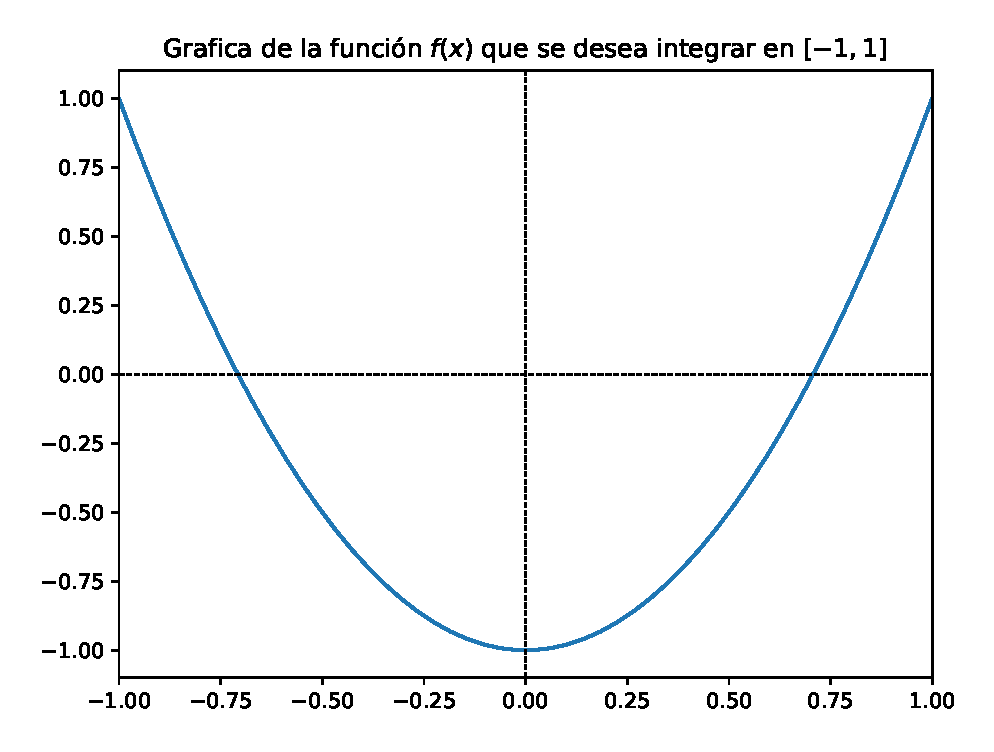
\includegraphics[scale=0.5]{Imagenes/integral_1_3_simpson.eps}
    \caption{Queremos calcular el valor del área debajo de la curva.}
\end{figure}
\end{frame}
\begin{frame}
\frametitle{Código para la solución}
Presentamos una propuesta para resolver el ejercicio, la función \funcionazul{Simpson13}, requiere de los argumentos
\setbeamercolor{item projected}{bg=blue!70!black,fg=yellow}
\setbeamertemplate{enumerate items}[circle]
\begin{enumerate}[<+->]
\item La función $f(x)$
\item Los intervalos de integración $[x_{0}, x_{f}]$
\item El valor $n$ del número de intervalos.
\end{enumerate}
\end{frame}
\begin{frame}[allowframebreaks, fragile]
\begin{lstlisting}[caption=Propuesta de código, style=FormattedNumber, basicstyle=\linespread{1.1}\ttfamily=\small, columns=fullflexible]
def Simpson_13_(f, x_0_, xf, n):
    n = n - n%2 # truncar al numero par mas cercano
     
    if n <= 0:
        n = 1
   
    h = (xf - x_0_)/n
    x = x_0_
   
    suma = 0
   
    for j in range(int(n/2)):
        suma += f(x) + 4. * f(x + h) + f(x + 2 * h)
        x += 2 * h
    return (h/3.) * suma

def f(x):
    return cos(2 * acos(x))

for i in range(1, 4):
    print ('Para n = {0:}'.format(i*2))
    print ('La integral vale {0:1.10f}'.format(Simpson_13_(f, -1., 1., i * 2)))
\end{lstlisting}
\end{frame}
\begin{frame}[fragile]
\frametitle{Solución en la terminal}
\begin{verbatim}
Para n = 2
La integral vale = -0.6666666667

Para n = 4
La integral vale = -0.6666666667

Para n = 6
La integral vale = -0.6666666667
\end{verbatim}
\end{frame}
\end{document}